\chapter{Perancangan}
\label{chap:design}
Berdasarkan analisis pada Bab 3, pada bab ini akan dipaparkan mengenai perancangan lojik basisdata, perancangan fisik basisdata, perancangan kelas MVC pada ODOO, diagram kelas, perancangan antar muka BI \textit{tool}, rancangan \textit{method-method} utama.

\section{Perancangan Lojik Basisdata}
Setelah pada bab 3 dijelaskan mengenai pemodelan basis data BI \textit{tool}, pada bagian ini akan digambarkan secara jelas rancangan struktur basisdata dari BI \textit{tool}. Rancangan basisdata ini merupakan impementasi dari skema \textit{star} menempatkan ba\_etl\_detail sebagai \textit{fact table}.\\
Keuntungan menerapkan skema \textit{star} adalah : 
\begin{enumerate}
	\item Lebih mudah dipahami sehingga memudahkan pengguna jika ingin mengembangkan BI \textit{tool} ini lebih lanjut.
	\item Secara teknis memudahkan \textit{developer} jika ingin mengembangkan fitur baru pada BI \textit{tool} ini.
	\item Efisien dalam mengakses data sehingga memudahkan untuk menampilkannya.
\end{enumerate}


\begin{figure}[H]
	\centering
	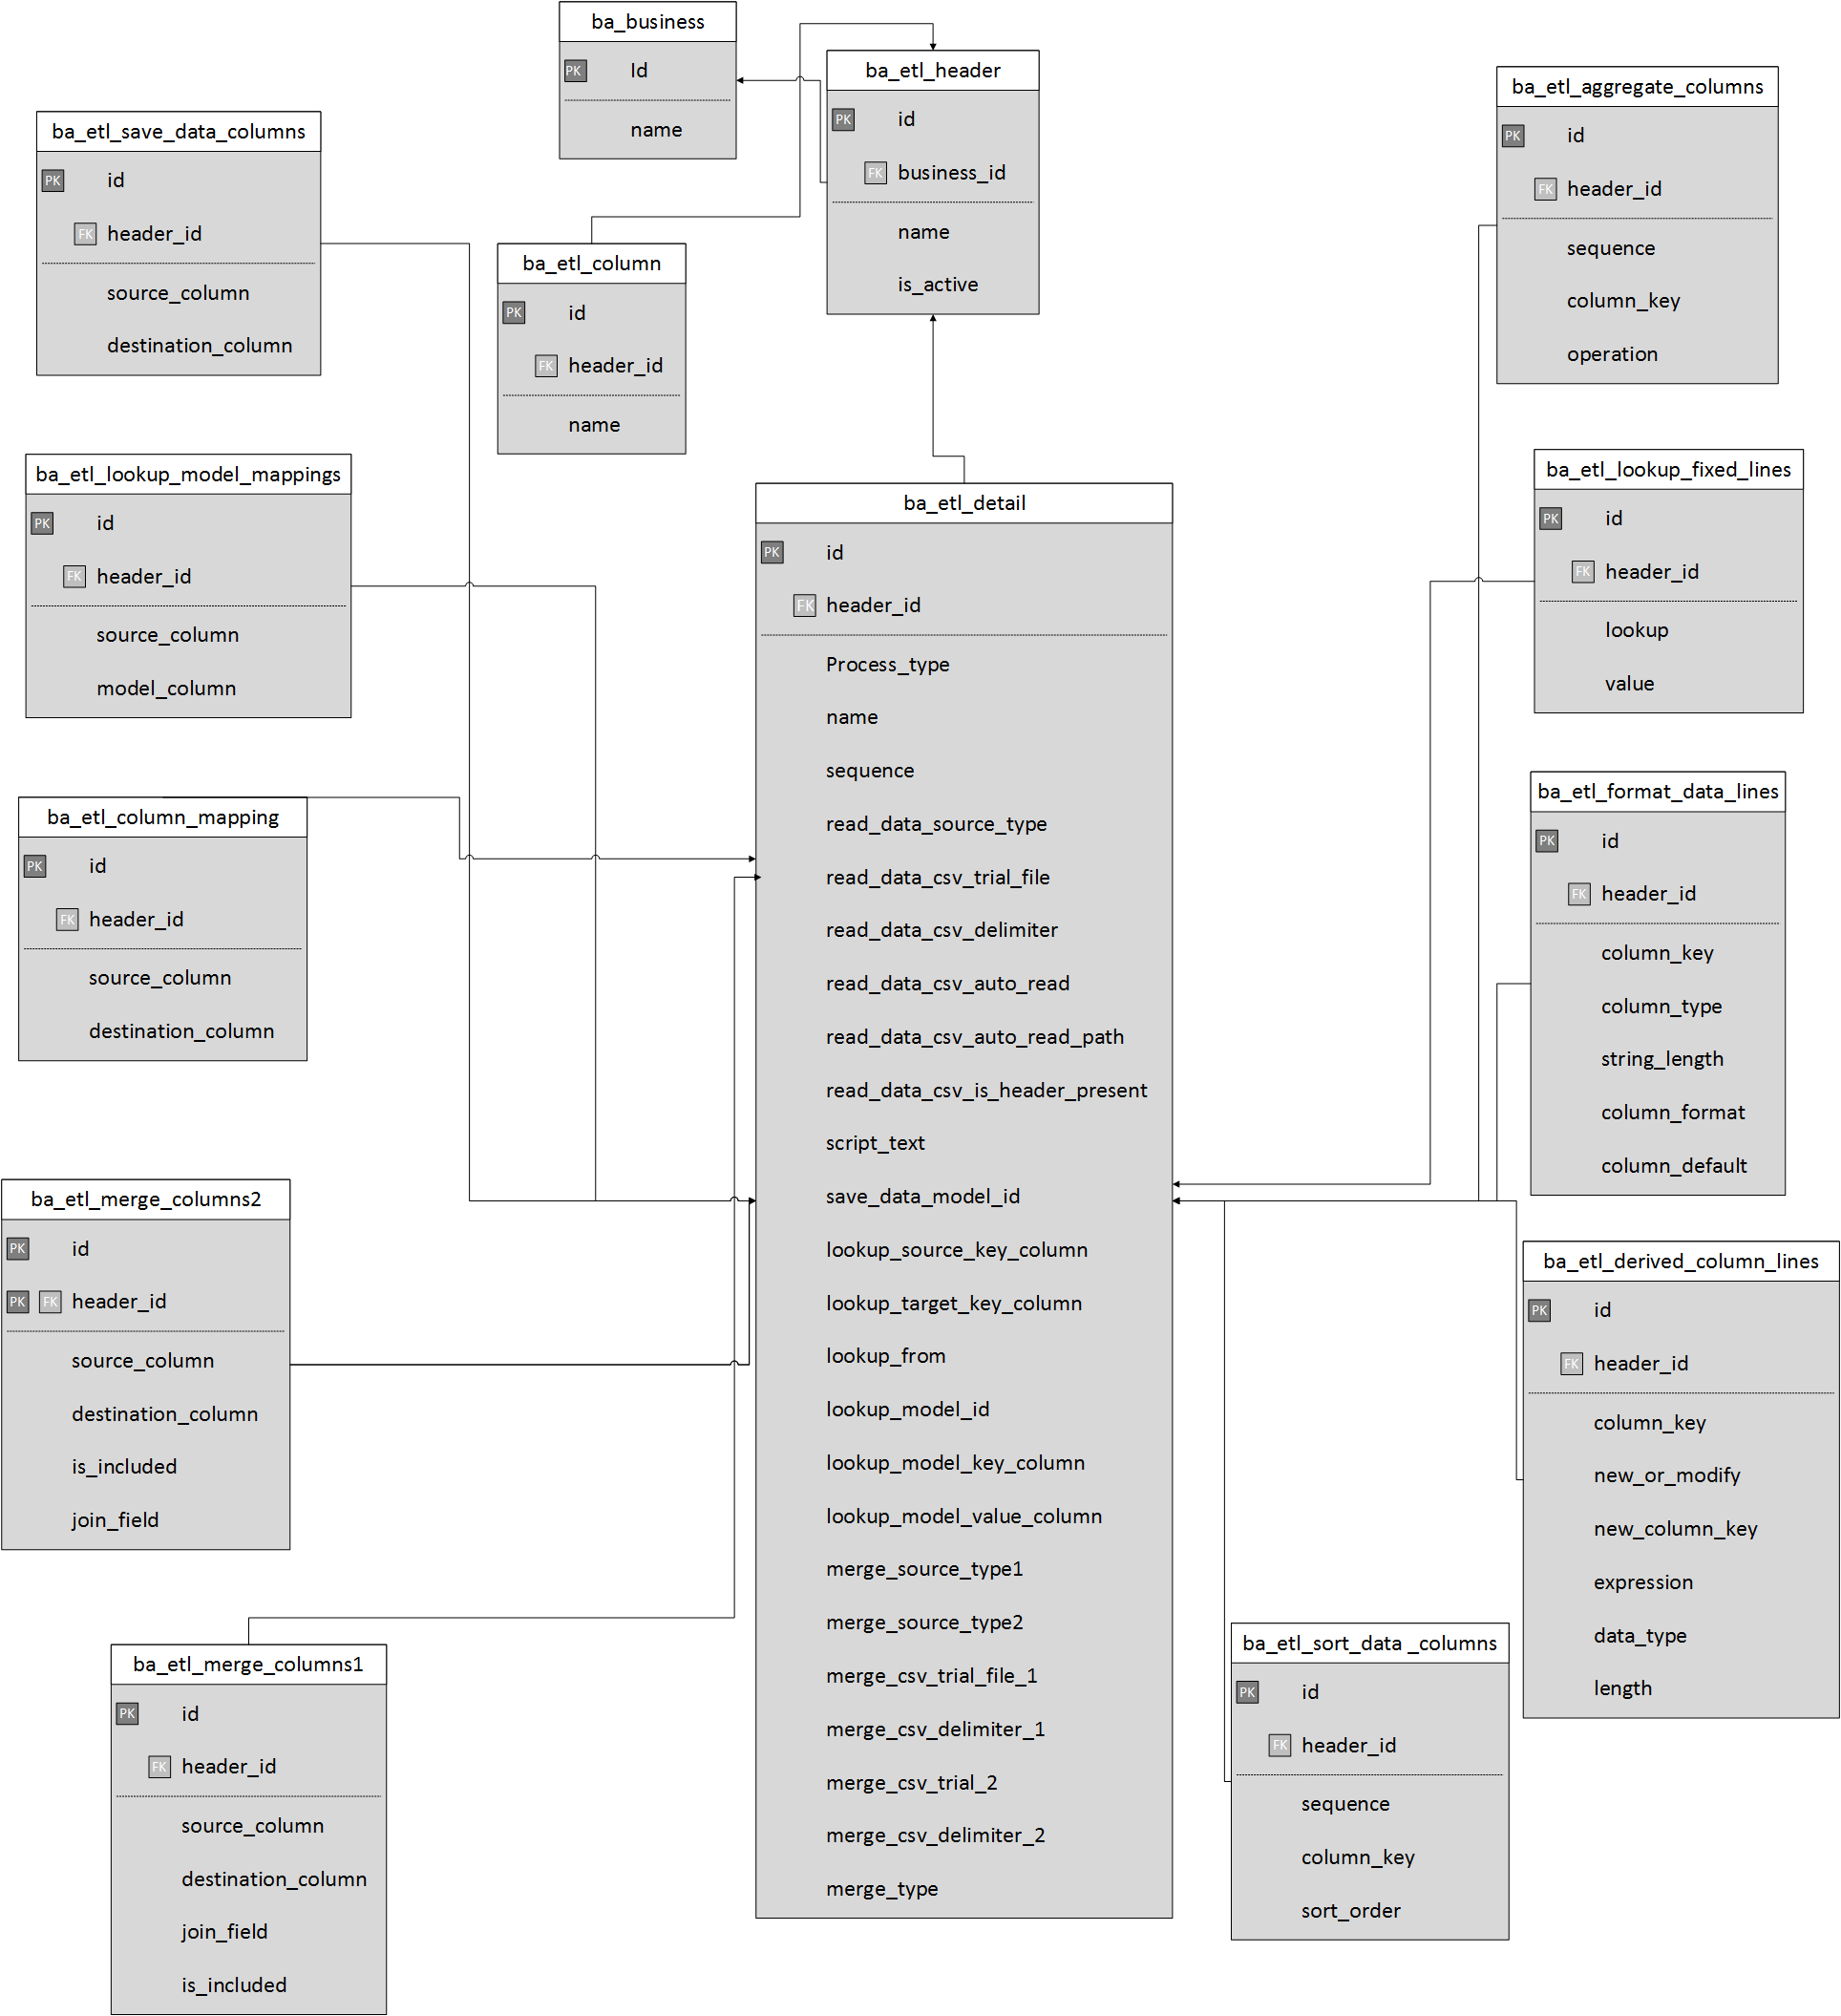
\includegraphics[scale=0.3]{Gambar/rancangan-basisdata-bi}
	\caption{Diagram Relational pada Basisdata BI \textit{tool}}
	\end{figure}
	
	\section{Perancangan Fisik Basisdata}
	Pada bagian sebelumnya telah digambarkan rancangan lojik basisdata BI \textit{tool}, berikut ini penjelasan detil kolom-kolom dalam tabel tersebut.
	\begin{table}[H]
	\centering
		\caption{Tabel \textit{ba\_bussiness}}
		\begin{tabular}{ | c | c| c | c | }
			\hline
				Field & Tipe & Panjang & Constraint \\ \hline \hline
			id & NUMBER & 10 & NOT NULL; PRIMARY KEY  \\ \hline
			name & VARCHAR & 200 & NOT NULL  \\ 		\hline 
		\end{tabular}
\end{table}

\begin{table}[H]
	\centering
		\caption{Tabel \textit{ba\_etl\_header}}
		\begin{tabular}{ | c | p{4cm} | c | p{4cm} |}
			\hline
				Field & Tipe & Panjang & Constraint \\ \hline \hline
			id & NUMBER & 10 & NOT NULL; PRIMARY KEY  \\ \hline
			bussiness\_id & MANY2ONE ba\_business& & NOT NULL; FOREIGN KEY  \\ \hline 
			name & VARCHAR & 200 & NOT NULL \\ \hline 
			is\_active & BOOLEAN &  & DEFAULT TRUE  \\ \hline 
		\end{tabular}
\end{table}

\begin{table}[H]
	\centering
		\caption{Tabel \textit{ba\_etl\_detail}}
		\begin{tabular}{ |c|p{3cm}|c|p{3cm}| }
			\hline
				Field & Tipe & Panjang & Constraint \\ \hline \hline
			id & NUMBER & 10 & NOT NULL; PRIMARY KEY  \\ \hline
			header\_id & MANY2ONE ba\_etl\_header& & NOT NULL; FOREIGN KEY \\ \hline 
			process\_type & ENUM(read\_data, format\_data, lookup, sort\_data, derived\_column, script, merge, aggregate, sort\_data, save\_data)&  & NOT NULL \\ \hline 
			name & VARCHAR &  & NOT NULL \\ \hline 
			sequence & INTEGER &  & NOT NULL  \\ \hline 
			read\_data\_source\_type & ENUM(CSV) & 20 & \\ \hline
			read\_data\_csv\_trial\_file & BINARY &  & \\ \hline 
			read\_data\_csv\_delimiter & VARCHAR & 2 & \\ \hline 
			read\_data\_csv\_auto\_read & BOOLEAN &  & \\ \hline 
			read\_data\_csv\_auto\_read\_path & VARCHAR &  & \\ \hline 
			read\_data\_csv\_is\_header\_present & BOOLEAN &  & DEFAULT TRUE \\ \hline 
			script\_text & TEXT &  & \\ \hline 
			save\_data\_model\_id & MANY2ONE ir\_model &  & \\ \hline 
			lookup\_source\_key\_column & MANY2ONE ba\_etl\_columns &  & \\ \hline
			lookup\_target\_key\_column & varchar & 64 & \\ \hline
			lookup\_from & ENUM(fixed, existing\_table) &  & \\ \hline
			lookup\_model\_id & MANY2ONE ir\_model &  & \\ \hline
			lookup\_model\_key\_column & VARCHAR & 64 & \\ \hline
			lookup\_model\_value\_column & VARCHAR & 64 & \\ \hline
			merge\_source\_type\_1 & ENUM(CSV) &  & \\ \hline
			merge\_source\_type\_2 & ENUM(CSV) &  & \\ \hline
			merge\_csv\_trial\_file\_1 & BINARY &  & \\ \hline
			merge\_csv\_trial\_file\_2 & BINARY &  & \\ \hline
			merge\_csv\_delimiter\_1 & VARCHAR & 3 & \\ \hline
			merge\_csv\_delimiter\_2 & VARCHAR & 3 & \\ \hline
			merge\_type & ENUM(left, right, inner) &  & \\ \hline
		\end{tabular}
\end{table}

\begin{table}[H]
	\centering
		\caption{Tabel \textit{ba\_etl\_columns}}
		\begin{tabular}{ | c | p{4cm} | c | p{4cm} |}
			\hline
				Field & Tipe & Panjang & Constraint \\ \hline \hline
			id & NUMBER & 10 & NOT NULL; PRIMARY KEY  \\ \hline
			header\_id & MANY2ONE ba\_etl\_header & &  FOREIGN KEY  \\ \hline 
			name & VARCHAR & 64 & \\ \hline 
		\end{tabular}
\end{table}

\begin{table}[H]
	\centering
		\caption{Tabel \textit{ba\_etl\_columns\_mapping}}
		\begin{tabular}{ | c | p{4cm} | c | p{4cm} |}
			\hline
				Field & Tipe & Panjang & Constraint \\ \hline \hline
			id & NUMBER & 10 & NOT NULL; PRIMARY KEY  \\ \hline
			header\_id & MANY2ONE ba\_etl\_detail & & NOT NULL; FOREIGN KEY  \\ \hline 
			source\_column & VARCHAR & 64 &  \\ \hline 
			detination\_column & VARCHAR & 64 &  \\ \hline 
		\end{tabular}
\end{table}

\begin{table}[H]
	\centering
		\caption{Tabel \textit{ba\_etl\_format\_data\_lines}}
		\begin{tabular}{ | c | p{4cm} | c | p{4cm} |}
			\hline
				Field & Tipe & Panjang & Constraint \\ \hline \hline
			id & NUMBER & 10 & NOT NULL; PRIMARY KEY  \\ \hline
			header\_id & MANY2ONE ba\_etl\_detail & & NOT NULL; FOREIGN KEY  \\ \hline 
			column\_key & MANY2ONE ba\_etl\_columns &  & NOT NULL  \\ \hline 
			column\_type & ENUM(char, integer, float, date, datetime, boolean, selection) &  &  \\ \hline 
		string\_length & INTEGER &  &  \\ \hline
		column\_format & VARCHAR & 50 &  \\ \hline
		column\_default & VARCHAR & 500  &  \\ \hline
		\end{tabular}
\end{table}

\begin{table}[H]
	\centering
		\caption{Tabel \textit{ba\_etl\_sort\_data\_columns}}
		\begin{tabular}{ | c | p{4cm} | c | p{4cm} |}
			\hline
				Field & Tipe & Panjang & Constraint \\ \hline \hline
			id & NUMBER & 10 & NOT NULL; PRIMARY KEY  \\ \hline
			header\_id & MANY2ONE ba\_etl\_detail & & NOT NULL; FOREIGN KEY  \\ \hline 
			sequence & INTEGER &  & NOT NULL  \\ \hline 
			column\_key & MANY2ONE ba\_etl\_columns &  &  \\ \hline 
		sort\_order & ENUM(asc, desc) &  & DEFAULT ASC  \\ \hline
		\end{tabular}
\end{table}

\begin{table}[H]
	\centering
		\caption{Tabel \textit{ba\_etl\_derived\_column\_lines}}
		\begin{tabular}{ | c | p{4cm} | c | p{4cm} |}
			\hline
				Field & Tipe & Panjang & Constraint \\ \hline \hline
			id & NUMBER & 10 & NOT NULL; PRIMARY KEY  \\ \hline
			header\_id & MANY2ONE ba\_etl\_detail & & NOT NULL; FOREIGN KEY  \\ \hline 	
			column\_key & MANY2ONE ba\_etl\_columns &  &   \\ \hline
			new\_or\_modify  & ENUM(new, modify) &  & DEFAULT NEW\\ \hline
			new\_column\_key & VARCHAR & 64 &  \\ \hline 
		expression & TEXT &  &  \\ \hline
		data\_type & ENUM(char, integer, float, date, datetime, boolean, selection) & &  \\ \hline
		length & INTEGER &   &  \\ \hline
		\end{tabular}
\end{table}

\begin{table}[H]
	\centering
		\caption{Tabel \textit{ba\_etl\_lookup\_fixed\_lines}}
		\begin{tabular}{ | c | p{4cm} | c | p{4cm} |}
			\hline
				Field & Tipe & Panjang & Constraint \\ \hline \hline
			id & NUMBER & 10 & NOT NULL; PRIMARY KEY  \\ \hline
			header\_id & MANY2ONE ba\_etl\_detail & & NOT NULL; FOREIGN KEY  \\ \hline 
			lookup & VARCHAR & 500  &  \\ \hline 
			value & VARCHAR & 500  &  \\ \hline 
		\end{tabular}
\end{table}

\begin{table}[H]
	\centering
		\caption{Tabel \textit{ba\_etl\_save\_data\_column}}
		\begin{tabular}{ | c | p{4cm} | c | p{4cm} |}
			\hline
				Field & Tipe & Panjang & Constraint \\ \hline \hline
			id & NUMBER & 10 & NOT NULL; PRIMARY KEY  \\ \hline
			header\_id & MANY2ONE ba\_etl\_detail & & \\ \hline 
			source\_column & MANY2ONE ba\_etl\_column & &  \\ \hline 
			destination\_column & VARCHAR & 64  &  \\ \hline  
		\end{tabular}
\end{table}

\begin{table}[H]
	\centering
		\caption{Tabel \textit{ba\_etl\_lookup\_model\_mappings}}
		\begin{tabular}{ | c | p{4cm} | c | p{4cm} |}
			\hline
				Field & Tipe & Panjang & Constraint \\ \hline \hline
			id & NUMBER & 10 & NOT NULL; PRIMARY KEY  \\ \hline
			header\_id & MANY2ONE ba\_etl\_detail & & \\ \hline 
			source\_column & MANY2ONE ba\_etl\_column & &  \\ \hline 
			destination\_column & VARCHAR & 64  &  \\ \hline  
		\end{tabular}
\end{table}

\begin{table}[H]
	\centering
		\caption{Tabel \textit{ba\_etl\_merge\_columns\_1}}
		\begin{tabular}{ | c | p{4cm} | c | p{4cm} |}
			\hline
				Field & Tipe & Panjang & Constraint \\ \hline \hline
			id & NUMBER & 10 & NOT NULL; PRIMARY KEY  \\ \hline
			header\_id & MANY2ONE ba\_etl\_detail & & \\ \hline 
			source\_column & VARCHAR & 64 &  \\ \hline 
			destination\_column & VARCHAR & 64  &  \\ \hline
			is\_included & BOOLEAN &  & DEFAULT 1 \\ \hline
			join\_field & VARCHAR & 64  &  \\ \hline
		\end{tabular}
\end{table}

\begin{table}[H]
	\centering
		\caption{Tabel \textit{ba\_etl\_merge\_columns\_2}}
		\begin{tabular}{ | c | p{4cm} | c | p{4cm} |}
			\hline
				Field & Tipe & Panjang & Constraint \\ \hline \hline
			id & NUMBER & 10 & NOT NULL; PRIMARY KEY  \\ \hline
			header\_id & MANY2ONE ba\_etl\_detail & & \\ \hline 
			source\_column & VARCHAR & 64 &  \\ \hline 
			destination\_column & VARCHAR & 64  &  \\ \hline
			is\_included & BOOLEAN &  & DEFAULT 1 \\ \hline
			join\_field & VARCHAR & 64  &  \\ \hline
		\end{tabular}
\end{table}

\begin{table}[H]
	\centering
		\caption{Tabel \textit{ba\_etl\_aggregate\_columns}}
		\begin{tabular}{ | c | p{4cm} | c | p{4cm} |}
			\hline
				Field & Tipe & Panjang & Constraint \\ \hline \hline
			id & NUMBER & 10 & NOT NULL; PRIMARY KEY  \\ \hline
			header\_id & MANY2ONE ba\_etl\_detail & & \\ \hline 
			sequence & INTEGER &  &  \\ \hline 
			column\_key & MANY2ONE ba\_etl\_columns &  &  \\ \hline
			operation & ENUM(none, count, sum, avg, max, min, group\_by) &  &\\ \hline
		\end{tabular}
\end{table}

\section{Diagram Kelas}
Berikut ini merupakan gambaran diagram kelas dari BI \textit{tool}. Setiap kelas pada diagram ini meng-\textit{extend} kelas osv yang merupakan bawaan dari \textit{framework} ODOO.

\begin{figure}[h]
	\centering
	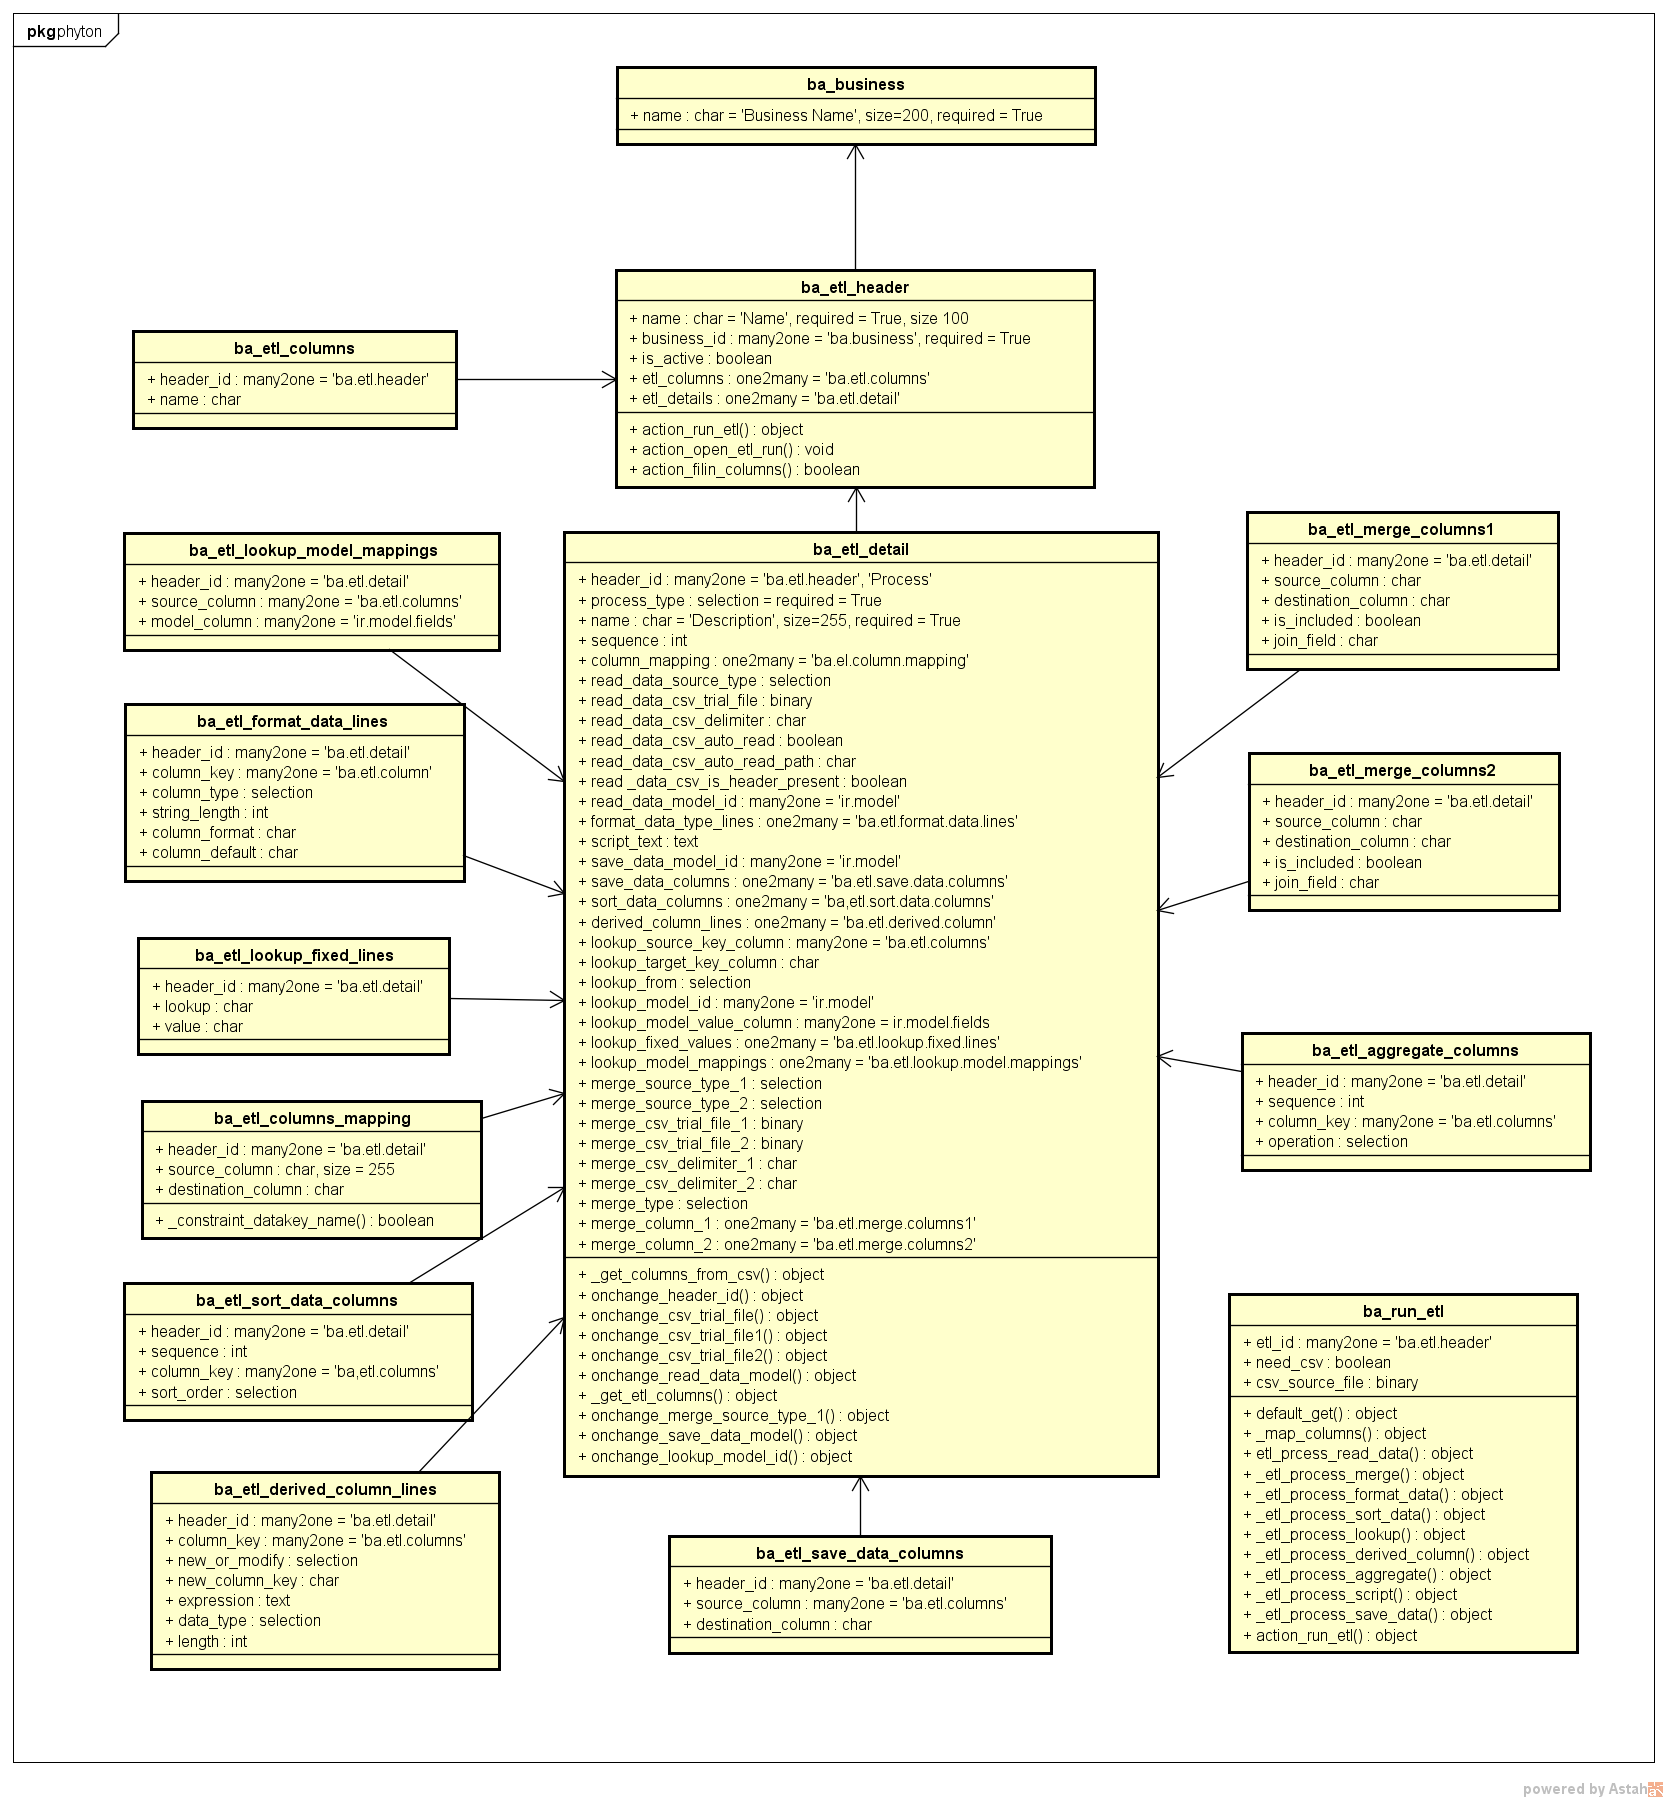
\includegraphics[scale=0.4]{Gambar/Class-Diagram-bi-tool}
	\caption{Struktur kelas diagram BI \textit{tool}}
	\end{figure}
	
	
	\begin{table}[H]
	\centering
		\caption{Tabel Kelas \textit{ba\_bussiness}}
		\begin{tabular}{ | c | c|}
			\hline
				\multicolumn{2}{|c|}{Atribut}\\ \hline 
				Nama atribut & Tipe Data\\ \hline
			name & CHAR(200)\\ \hline
		\end{tabular}
\end{table}

\begin{table}[H]
	\centering
		\caption{Tabel Kelas \textit{ba\_etl\_header}}
		\begin{tabular}{ | c | c|}
			\hline
				\multicolumn{2}{|c|}{Atribut}\\ \hline 
				Nama atribut & Tipe Data\\ \hline
			name & CHAR(100)\\ \hline
			business\_id & MANY2ONE('ba.business')\\ \hline
			is\_active & BOOLEAN\\ \hline
			etl\_columns & ONE2MANY('ba.etl.columns')\\ \hline
			etl\_detail & ONE2MANY('ba.etl.detail')\\ \hline
			\multicolumn{2}{|c|}{Method}\\ \hline 
			\multicolumn{2}{|l|}{action\_run\_etl()}\\ \hline 
			\multicolumn{2}{|l|}{action\_open\_etl\_run()}\\ \hline
			\multicolumn{2}{|l|}{action\_fillin\_columns()}\\ \hline
		\end{tabular}
\end{table}

\begin{table}[H]
	\centering
		\caption{Tabel Kelas \textit{ba\_etl\_columns}}
		\begin{tabular}{ | c | c|}
			\hline
				\multicolumn{2}{|c|}{Atribut}\\ \hline 
				Nama atribut & Tipe Data\\ \hline
			header\_id & MANY2ONE('ba.etl.header')\\ \hline
			name & CHAR\\ \hline
		\end{tabular}
\end{table}

\begin{table}[H]
	\centering
		\caption{Tabel Kelas \textit{ba\_etl\_detail}}
		\begin{tabular}{ | c | c|}
			\hline
				\multicolumn{2}{|c|}{Atribut}\\ \hline 
				Nama atribut & Tipe Data\\ \hline
			header\_id & MANY2ONE('ba.etl.header')\\ \hline
			process\_type & selection\\ \hline
			name & CHAR(255)\\ \hline
			sequence &  INT\\ \hline
			column\_mapping &  ONE2MANY('ba.el.column.mapping)\\ \hline
			read\_data\_source\_type & SELECTION\\ \hline
			read\_data\_csv\_trial\_file &  BINARY\\ \hline
			read\_data\_csv\_delimiter &  CHAR\\ \hline
			read\_data\_csv\_auto\_read &  BOOLEAN\\ \hline
			read\_data\_csv\_auto\_read\_path &  CHAR\\ \hline
			read\_data\_csv\_is\_header\_present &  BOOLEAN\\ \hline
			read\_data\_model\_id &  MANY2ONE('ir.model')\\ \hline
			format\_data\_type\_lines &  ONE2MANY('ba.etl.format.data.lines')\\ \hline
			script\_text &  TEXT\\ \hline
			save\_data\_model\_id &  MANY2ONE('ir.model')\\ \hline
			save\_data\_columns & ONE2MANY('ba.etl.save.data.columns')\\ \hline
			sort\_data\_columns &  ONE2MANY('ba.etl.sort.data.column')\\ \hline
			 derived\_column\_lines &  ONE2MANY('ba.etl.derived.column')\\ \hline
			lookup\_source\_key\_column &  MANY2ONE('ba.etl.columns')\\ \hline
			lookup\_target\_key\_column &  CHAR\\ \hline
			lookup\_from &  SELECTION\\ \hline
		  lookup\_model\_id &  MANY2ONE('ir.model')\\ \hline
			lookup\_model\_value\_column &  MANY2ONE(ir.model.fields)\\ \hline
			lookup\_fixed\_values &  ONE2MANY('ba.etl.lookup.fixed.lines')\\ \hline
			lookup\_model\_mappings &  ONE2MANY('ba.etl.lookup.model.mappings')\\ \hline
			merge\_source\_type\_1 &  SELECTION\\ \hline
			merge\_source\_type\_2 &  SELECTION\\ \hline
			merge\_csv\_trial\_file\_1 &  BINARY\\ \hline
			merge\_csv\_trial\_file\_2 &  BINARY\\ \hline
			merge\_csv\_delimiter\_1 &  CHAR\\ \hline
			merge\_csv\_delimiter\_2 &  CHAR\\ \hline
			merge\_type &  SELECTION\\ \hline
			merge\_column\_1 &  ONE2MANY('ba.etl.merge.columns1')\\ \hline
			merge\_column\_2 &  ONE2MANY('ba.etl.merge.columns2')\\ \hline
			\multicolumn{2}{|c|}{Method}\\ \hline 
			\multicolumn{2}{|l|}{get\_columns\_from\_csv(csv\_content, delimiter) }\\ \hline 
			\multicolumn{2}{|l|}{onchange\_header\_id(header\_id)}\\ \hline
			\multicolumn{2}{|l|}{onchange\_csv\_trial\_file(read\_data\_csv\_trial\_file, delimiter)}\\ \hline
			\multicolumn{2}{|l|}{onchange\_csv\_trial\_file1(merge\_csv\_trial\_file\_1, merge\_csv\_delimiter\_1)}\\ \hline
			\multicolumn{2}{|l|}{onchange\_csv\_trial\_file2(merge\_csv\_trial\_file\_2, merge\_csv\_delimiter\_2)}\\ \hline
			\multicolumn{2}{|l|}{onchange\_read\_data\_model(read\_data\_model\_id)}\\ \hline
			\multicolumn{2}{|l|}{get\_etl\_columns(header\_id)}\\ \hline
			\multicolumn{2}{|l|}{onchange\_merge\_source\_type\_1(header\_id, merge\_source\_type\_1)}\\ \hline
			\multicolumn{2}{|l|}{onchange\_save\_data\_model(save\_data\_model\_id)}\\ \hline
			\multicolumn{2}{|l|}{onchange\_lookup\_model\_id(lookup\_model\_id)}\\ \hline
			
		\end{tabular}
\end{table}

\begin{table}[H]
	\centering
		\caption{Tabel Kelas \textit{ba\_etl\_columns\_mapping}}
		\begin{tabular}{ | c | c|}
			\hline
				\multicolumn{2}{|c|}{Atribut}\\ \hline 
				Nama atribut & Tipe Data\\ \hline
				header\_id & MANY2ONE('ba.etl.detail')\\ \hline
				source\_column & CHAR(255)\\ \hline
				destination\_column & CHAR\\ \hline
				\multicolumn{2}{|c|}{Method}\\ \hline
				\multicolumn{2}{|l|}{constraint\_datakey\_name()}
		\end{tabular}
\end{table}
	
	\begin{table}[H]
	\centering
		\caption{Tabel Kelas \textit{ba\_etl\_format\_data\_lines}}
		\begin{tabular}{ | c | c|}
			\hline
				\multicolumn{2}{|c|}{Atribut}\\ \hline 
				Nama atribut & Tipe Data\\ \hline
				header\_id & MANY2ONE('ba.etl.detail')\\ \hline
				column\_key & MANY2ONE('ba.etl.column')\\ \hline
				column\_type & SELECTION\\ \hline
				string\_length & INT\\ \hline
				column\_format & CHAR(50)\\ \hline
				column\_default & CHAR(500)\\ \hline
		\end{tabular}
\end{table}

\begin{table}[H]
	\centering
		\caption{Tabel Kelas \textit{ba\_etl\_sort\_data\_columns}}
		\begin{tabular}{ | c | c|}
			\hline
				\multicolumn{2}{|c|}{Atribut}\\ \hline 
				Nama atribut & Tipe Data\\ \hline
				header\_id & MANY2ONE('ba.etl.detail')\\ \hline
				sequence & INT\\ \hline
				column\_key & MANY2ONE('ba.etl.column')\\ \hline
				sort\_order & SELECTION\\ \hline
		\end{tabular}
\end{table}

\begin{table}[H]
	\centering
		\caption{Tabel Kelas \textit{ba\_etl\_derived\_column\_lines}}
		\begin{tabular}{ | c | c|}
			\hline
				\multicolumn{2}{|c|}{Atribut}\\ \hline 
				Nama atribut & Tipe Data\\ \hline
				header\_id & MANY2ONE('ba.etl.detail')\\ \hline
				column\_key & MANY2ONE('ba.etl.column')\\ \hline
				new\_or\_modify  & SELECTION\\ \hline
				new\_column\_key & CHAR(64)\\ \hline
				expression & TEXT \\ \hline
				data\_type & SELECTION \\ \hline
				length & INT \\ \hline
		\end{tabular}
\end{table}

\begin{table}[H]
	\centering
		\caption{Tabel Kelas \textit{ba\_etl\_save\_data\_columns}}
		\begin{tabular}{ | c | c|}
			\hline
				\multicolumn{2}{|c|}{Atribut}\\ \hline 
				Nama atribut & Tipe Data\\ \hline
				header\_id & MANY2ONE('ba.etl.detail')\\ \hline
				source\_column & MANY2ONE('ba.etl.column')\\ \hline
				destination & CHAR(64)\\ \hline
		\end{tabular}
\end{table}

\begin{table}[H]
	\centering
		\caption{Tabel Kelas \textit{ba\_etl\_lookup\_fixed\_lines}}
		\begin{tabular}{ | c | c|}
			\hline
				\multicolumn{2}{|c|}{Atribut}\\ \hline 
				Nama atribut & Tipe Data\\ \hline
				header\_id & MANY2ONE('ba.etl.detail')\\ \hline
				lookup & CHAR\\ \hline
				value& CHAR\\ \hline
		\end{tabular}
\end{table}

\begin{table}[H]
	\centering
		\caption{Tabel Kelas \textit{ba\_etl\_lookup\_model\_mappings}}
		\begin{tabular}{ | c | c|}
			\hline
				\multicolumn{2}{|c|}{Atribut}\\ \hline 
				Nama atribut & Tipe Data\\ \hline
				header\_id & MANY2ONE('ba.etl.detail')\\ \hline
				source\_column & MANY2ONE('ba.etl.column')\\ \hline
				model\_column & MANY2ONE('ir.model.fields')\\ \hline
		\end{tabular}
\end{table}

\begin{table}[H]
	\centering
		\caption{Tabel Kelas \textit{ba\_etl\_merge\_columns1}}
		\begin{tabular}{ | c | c|}
			\hline
				\multicolumn{2}{|c|}{Atribut}\\ \hline 
				Nama atribut & Tipe Data\\ \hline
				header\_id & MANY2ONE('ba.etl.detail')\\ \hline
				source\_column & CHAR(64)\\ \hline
				destination\_column & CHAR(64)\\ \hline
				is\_included & BOOLEAN\\ \hline
				join\_field & CHAR\\ \hline
		\end{tabular}
\end{table}

\begin{table}[H]
	\centering
		\caption{Tabel Kelas \textit{ba\_etl\_merge\_columns2}}
		\begin{tabular}{ | c | c|}
			\hline
				\multicolumn{2}{|c|}{Atribut}\\ \hline 
				Nama atribut & Tipe Data\\ \hline
				header\_id & MANY2ONE('ba.etl.detail')\\ \hline
				source\_column & CHAR(64)\\ \hline
				destination\_column & CHAR(64)\\ \hline
				is\_included & BOOLEAN\\ \hline
				join\_field & CHAR\\ \hline
		\end{tabular}
\end{table}

\begin{table}[H]
	\centering
		\caption{Tabel Kelas \textit{ba\_etl\_aggregate\_columns}}
		\begin{tabular}{ | c | c|}
			\hline
				\multicolumn{2}{|c|}{Atribut}\\ \hline 
				Nama atribut & Tipe Data\\ \hline
				header\_id & MANY2ONE('ba.etl.detail')\\ \hline
				sequence & INT\\ \hline
				column\_key & MANY2ONE('ba.etl.columns')\\ \hline
				operation & SELECTION\\ \hline
		\end{tabular}
\end{table}

\begin{table}[H]
	\centering
		\caption{Tabel Kelas \textit{ba\_run\_etl}}
		\begin{tabular}{ | c | c|}
			\hline
				\multicolumn{2}{|c|}{Atribut}\\ \hline 
				Nama atribut & Tipe Data\\ \hline
				etl\_id & MANY2ONE('ba.etl.header')\\ \hline
				need\_csv & BOOLEAN\\ \hline
				csv\_source\_file & BINARY\\ \hline
				\multicolumn{2}{|c|}{Method}\\ \hline
				\multicolumn{2}{|l|}{default\_get(fields)}\\ \hline
				\multicolumn{2}{|l|}{map\_columns(source\_data, columns\_mapping)}\\ \hline
				\multicolumn{2}{|l|}{etl\_process\_read\_data(step\_info, raw\_data)}\\ \hline
				\multicolumn{2}{|l|}{etl\_process\_merge(step\_info, raw\_data)}\\ \hline
				\multicolumn{2}{|l|}{etl\_process\_format\_data(step\_info, raw\_data)}\\ \hline
				\multicolumn{2}{|l|}{etl\_process\_sort\_data(step\_info, raw\_data)}\\ \hline
				\multicolumn{2}{|l|}{etl\_process\_lookup(step\_info, raw\_data)}\\ \hline
				\multicolumn{2}{|l|}{etl\_process\_derived\_column(step\_info, raw\_data)}\\ \hline
				\multicolumn{2}{|l|}{etl\_process\_aggregate(step\_info, raw\_data)}\\ \hline
				\multicolumn{2}{|l|}{etl\_process\_script(step\_info, raw\_data)}\\ \hline
				\multicolumn{2}{|l|}{etl\_process\_save\_data(step\_info, raw\_data)}\\ \hline
				\multicolumn{2}{|l|}{action\_run\_etl(etl\_id)}\\ \hline
		\end{tabular}
\end{table}
